\chapter{Contextual Background}
\label{chap:context}

% {\bf A compulsory chapter, of roughly $5$ pages}
% \vspace{1cm}
%
% \noindent
% This chapter should describe the project context, and motivate each of the proposed aims and objectives. 
% Ideally, it is written at a fairly high-level, and easily understood by a reader who is technically competent but not an expert in the topic itself.

% In short, the goal is to answer three questions for the reader.
In this chapter, I aim to outline what bouldering is, why recreational intermediate boulderers were my target audience and test-population, the gaps in literature that this project aims to explore.
I also detail the four hypotheses that guided the development of both the app and the study, and outline some of the key challenges this project faced.

\section{The Problem Being Investigated}
\subsection{Indoor Bouldering}
For the purpose of this project, I will be studying how interacting with data affects indoor boulderers.

\subsubsection{What}
Bouldering is a sub-genre of climbing where the routes are generally quite short (under 5m), so no ropes or gear are required, only a soft crash-mat for safety.
\begin{figure}[h]
\centering
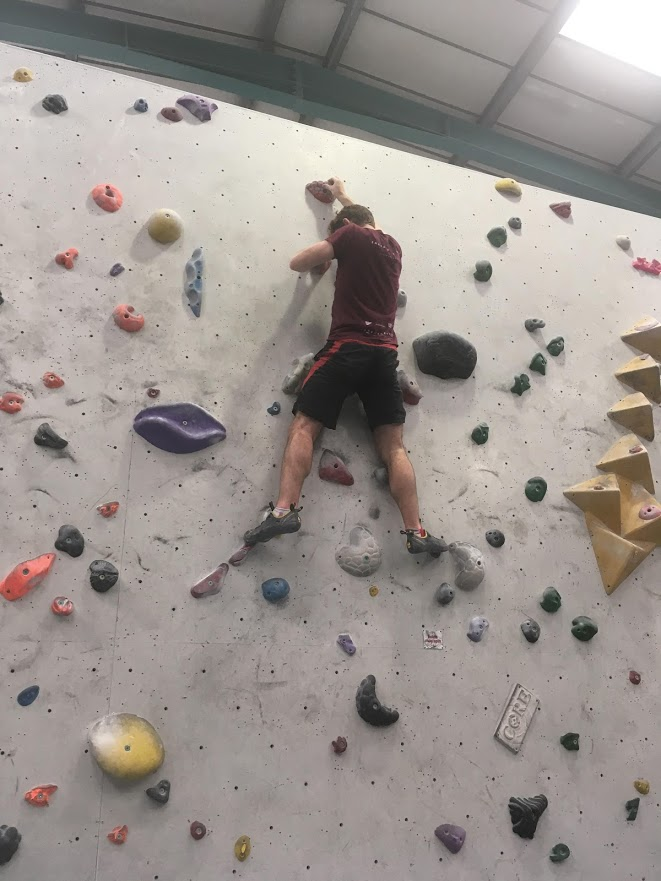
\includegraphics[width=4cm]{imgs/boulder}
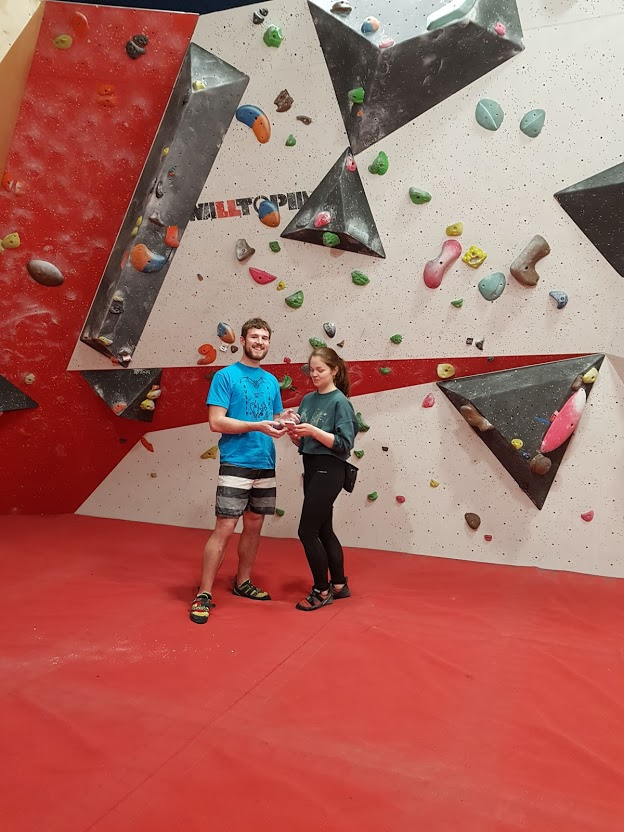
\includegraphics[width=4cm]{imgs/wall}
\caption{Example images of a bouldering wall}
\label{fig:playstore}
\end{figure}

Many indoor bouldering ``gyms" have opened in the past decade, with the low requirements for kit and more social environment being mentioned as some reasons for this growth~\cite{socialclimb}.

\subsubsection{Why}
Studying an indoor variant of climbing was chosen as it is weather in-dependant (a useful factor for a studying being conducted in the winter-spring seasons) and also because it was a lot more accessible for both me and my potential testers, with three locations across Bristol, all within easy cycling distance of the university.
This meant that many more test sessions could take place, between two and four three-hour sessions per week, which is much more than would have been possible with a drive out to a nearby rock-face.

Another reason indoor climbing (and the bouldering sub-type in particular) was chosen is because it usually involves shorter, slightly harder routes, with participants often discussing the climbs between attempts.
In addition, the shorter routes are easily visible from the ground, with fairly consistent lighting, potentially allowing a stationary camera-equipped device to observe the entire climb in-frame.



\subsubsection{Grades}
As a sport, the goal of climbing is to ascend (go up) or traverse (go across) a wall, from the ground to an end-point.

Some of these routes are more difficult than others, and so they can be ``graded" in various ways to indicate to other climbers the relative difficulty.
This difficulty is generally subjective, and is usually a combination of: the type and convenience of the holds, the distance between holds, and the incline of the wall.
Some people use this as just an indicator for which climbs they are likely to have the most fun on, and other use this as a tool for measuring their progression, trying to climb the highest grade they can.
Climbing routes that are easier than a persons maximum ability offers an opportunity to refine and hone strength and technique before attempting harder-graded climbs.

There are a variety of ways of grading routes.
Often bouldering uses a ``$V$" system, with $V0$ being easy beginner-orientated climbs, and $V7$ being an expert-level route.
In the old outdoor bouldering, this was determined by discussion and opinions on various natural holes in rocks, but in modern indoor bouldering gyms, climbing routes are designed, or ``set" with all the hand- and foot-holds being made of a certain coloured plastic, and that colour will signify it's difficulty.



\subsection{Intermediate-level Climbers}
To further help narrow the scope of the project, I decided to aim a potential product or interactive device on a typical intermediate climber.
This is because beginners often progress very quickly with just \textit{more time} spent climbing, and expert-level climbers often have their own coaches to aid in their growth, whilst a large number of intermediate climbers, who want to improve, maybe don't know what they need to do, and get no feedback from their current climbing.

For many intermediate boulderers who are facing a plateau in their progression, they currently face two options: either to continue climbing a lot at a low grade, hoping they gradually build up the strength and technique required to break through and climb harder; or to pay (quite a lot of) money for a private coach who can analyse their technique and give them precise feedback on how to improve.

Therefore from a climbing-improvement perspective, the product I was aiming to build could either incentivise climbing lower-grade with a high-volume, or give feedback on technique, or both.



\section{Importance of Topic}
% Second, why is the topic important, or rather why should the reader care about it?

% For example,
% why there is a need for this project
% (e.g., lack of similar software or deficiency in existing software),
% who will benefit from the project and in what way
% (e.g., end-users, or software developers)
% what work does the project build on and why is the selected approach either important and/or interesting
% (e.g., fills a gap in literature, applies results from another field to a new problem).


There is currently no lightweight device, product or app in the market that is aimed at helping intermediate climbers see data and progress in their climbing.
As will be further discussed in Chapter~\ref{chap:technical}, academic research has thus-far focused on very specialised hardware or custom-built climbing-walls, with little attention on something smaller or lightweight that is highly-accessible for every climber to use.


In conducting a user-centred iterative design to discover what kind of data interaction is most useful for intermediate climbers, I have both built a product that is fit-for-purpose, and have begun exploring what is an as-of-yet under-studied area in Human-Computer Interaction:
In-field user studies that aim to capture the view and use-patterns of the majority of boulderers.



\section{Hypotheses}
Along with developing a product, from a HCI perspective I also wanted to see how climbers interact with a more modern product or app.
Many climbers either ``just climb", leaving their phone in the lockers, or if they do track it they simply list which climbs they have completed in a logbook or logging-app, and there has been little-to-no research in the computerisation of mainstream climbing aids thus far.
Does the adding of some measurements and metrics aid a climber in the long run,
either by making climbing more fun and therefore causing them to go train more often, or does the frequency not change as much as the effectiveness of the training itself - instead of aimlessly climbing with a vague goal of ``getting better", does providing quantitative analysis of the climbs completed give more of a focus to the sessions that a climber does?


With these thoughts in mind, I formulated four key hypotheses to explore:
\begin{enumerate}
    \item Augmenting a climbing session with a live-feed of data analytics will positively impact climbing technique.
    \item A lightweight, low-cost and simple-to-use product will be popular among intermediate climbers who are serious enough to want to improve, but not so serious they want to pay for coaching.
    \item Seeing a ``score" that rates climbing technique will enable gamification and fun, both for individuals and within groups.
    \item Providing more data to climbers will enable more focused progression tracking and goal-oriented training.
\end{enumerate}



\section{Central Challenges}
% Finally, what are the central challenges involved and why are they significant?
One central challenge of the project was to iteratively develop a useful product that fits the needs of local indoor intermediate boulderers.
The associated second central challenge was the required testing, analysis and understanding of how the augmentation of live data analytics can aid a climber's progress or enjoyment.


With these initial goals, after months of study and through four major iteration-cycles, I developed an app that can record, share, and match accelerometer data and video recordings taken from a variety of devices at different times.
This was the third major challenge - alongside designing a product and investigating its impact on users, actually coding and publishing a feature-rich app that is reliable and fast on a range of devices was a big challenge.


Sub-challenges included:
\begin{enumerate}
\item designing a series of metrics that are useful and consistently comparable between climbs, \item exploring the video-analysis of climbing technique,
\item constant user testing and re-evaluation of goals, quickly developing features in time for a thrice-weekly in-field testing session at the wall,
\item ethical considerations of developing a product that advises people whilst they perform an inherently risky sport - both during the development of ideas, and the two full academic-ethics applications
\item running a series of longer-term user-analyses and interviews at the end of the project, to further explore the impact of using the completed app, then conducting a thematic analysis over the transcripts of the interviews.
\end{enumerate}
